\documentclass{tufte-handout}

\title{4.1 Exponential functions}

\author[AW]{Ammon Washburn}

\usepackage{graphicx} % allow embedded images
  \setkeys{Gin}{width=\linewidth,totalheight=\textheight,keepaspectratio}
  \graphicspath{{graphics/}} % set of paths to search for images
\usepackage{amsmath}  % extended mathematics
\usepackage{booktabs} % book-quality tables
\usepackage{units}    % non-stacked fractions and better unit spacing
\usepackage{multicol} % multiple column layout facilities
\usepackage{lipsum}   % filler text
\usepackage{enumerate}
\usepackage{wrapfig}
\usepackage{fancyvrb} % extended verbatim environments
  \fvset{fontsize=\normalsize}% default font size for fancy-verbatim environments
  \usepackage{tikz}

% Standardize command font styles and environments
\newcommand{\doccmd}[1]{\texttt{\textbackslash#1}}% command name -- adds backslash automatically
\newcommand{\docopt}[1]{\ensuremath{\langle}\textrm{\textit{#1}}\ensuremath{\rangle}}% optional command argument
\newcommand{\docarg}[1]{\textrm{\textit{#1}}}% (required) command argument
\newcommand{\docenv}[1]{\textsf{#1}}% environment name
\newcommand{\docpkg}[1]{\texttt{#1}}% package name
\newcommand{\doccls}[1]{\texttt{#1}}% document class name
\newcommand{\docclsopt}[1]{\texttt{#1}}% document class option name
\newenvironment{docspec}{\begin{quote}\noindent}{\end{quote}}% command specification environment

\newtheorem{mydef}{Definition}
\providecommand{\floor}[1]{\left \lfloor #1 \right \rfloor }

\begin{document}
\maketitle

\begin{abstract}
We will learn the properties of exponential functions and how to use them in modeling
\end{abstract}

\section{Exponential power properties}

\begin{align*}
a^m a^n & = a^{m+n}  & \textrm{Add the exponents} \\
\frac{a^m}{a^n} & =a^{m-n} & \textrm{Subtract the exponents} \\
(a^m)^n & = a^{mn} & \textrm{Multiply the exponents} \\
(ab)^n & = a^nb^n & \textrm{Distribute the exponents} \\
\bigg ( \frac{a}{b} \bigg )^n & = \frac{a^n}{b^n} & \textrm{Distribute the exponents}
\end{align*}

Word of warning: $a^{m^n} \neq (a^m)^n$.  Let $a=2$, $m=1$, $n=2$ as a counter-example.

\section{Exponential functions}
An exponential function is where your input is a power of some base.  What your graph looks like depends on the base.  For a simple exponential function of the form $f(x) = a^x$ we get the following properties.

\begin{figure}
\centering
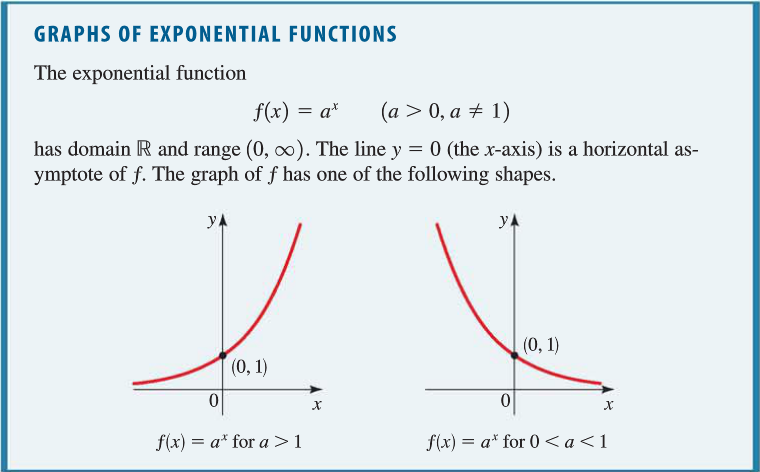
\includegraphics[width=\linewidth]{ExponentialGraphs.png}
\end{figure}

\subsection{Finding the equation given two points}
Say you have a simple exponential function that has been stretched or compressed vertically.  $f(x) = C b^x$.  How can you figure out the graph from two points?

If you have the y-intercept $(0,a)$ then $C=a$.  If you have another point then you plug into the equation and solve for $b$.

Example: Find the equation for the exponential function $g(x) = C b^x$ passing through the points $(0,2)$ and $(2,18)$.

Answer: $g(x) = 2 (3)^x$.

Example: Find the equation for the exponential function $h(x) = C b^x$ passing through the points $(1,6)$ and $(2,12)$.

Answer: $h(x) = 3 (2)^x$

\subsection{Transformations on the basic exponential function}

We learned about vertical stretching and compressing.  How does the properties of the simple exponential change under other transformations?

Shifting up or down by $a$? That changes the horizontal asymptote to be $y=a$ and the range to be $[a,\infty)$.

Reflecting over the x-axis? That changes the range to be $(-\infty,0]$.

Reflecting over the y-axis? That means our $b$ becomes $\frac{1}{b}$.

Horizontal shifting? This is harder to see since an exponential looks similar in every interval.  You can see that the y-intercept changes so it is like a stretch or a compression

\subsection{Compound interest}

\begin{mydef}
The model for representing the accumulated money $A(t)$ as a function of years $t$ with initial investment Pis given by the following equation: $A(t) = P(1 + \frac{r}{n})^{nt}$ where $r$ is the interest rate compounded $n$ times during the year
\end{mydef}

Make sure you know what compounded daily, weekly, etc mean in terms of n.

Example:

You are given the option to invest \$3000 in an account that pays 2.5\% compounded either yearly or daily.  Which one will generate more money after 2 years?

Answer: Compounded daily is better.


\end{document}